\chapter{Virtualization}
In this chapter we will be talking about virtualization, which is an activity aiming to create replacements for real resources, which have the same functionalities and external interfaces of their counterpart, but different attributes.

Virtualization, emulation and simulation are similar concepts that hide very important differences, we will be exploring them in the following.
\begin{itemize}
    \item Emulation: We use a system to execute another operating system (the concept can also be downscaled to APIs and single functions) that was not developed for the specific machine.

    Emulation can be really helpful because we can use it to run old operating systems on different hardware platforms or we can use it to read from memorization devices that we no longer have or no longer work.
    \item Simulation: An application allowing to execute old programs defined for different platforms on modern machines and it replicates the behaviour of a system. It's like a software emulation.

    Emulation is slower but precise while simulation is fast but less precise. We use simulation (or software emulation) to run old games on our smartphones.
    \item High level emulation is an intermediate between emulation and simulation, they recreate the functionalities of an emulated system using similar or equivalent functions in the emulating system. Since is an intermediate level between emulation and simulation it's slower than simulation but faster than emulation.
    \item Virtualization: the technique for using resources and devices in a functional way without considering their physical layout.

    In the world of virtualization a Virtual Machine is a container with software based CPU, RAM and HDD and network connection. We have a certain level of transparency because an OS or an application do not distinguish between a virtual and a physical machine.
\end{itemize}
\begin{figure}
    \centering
    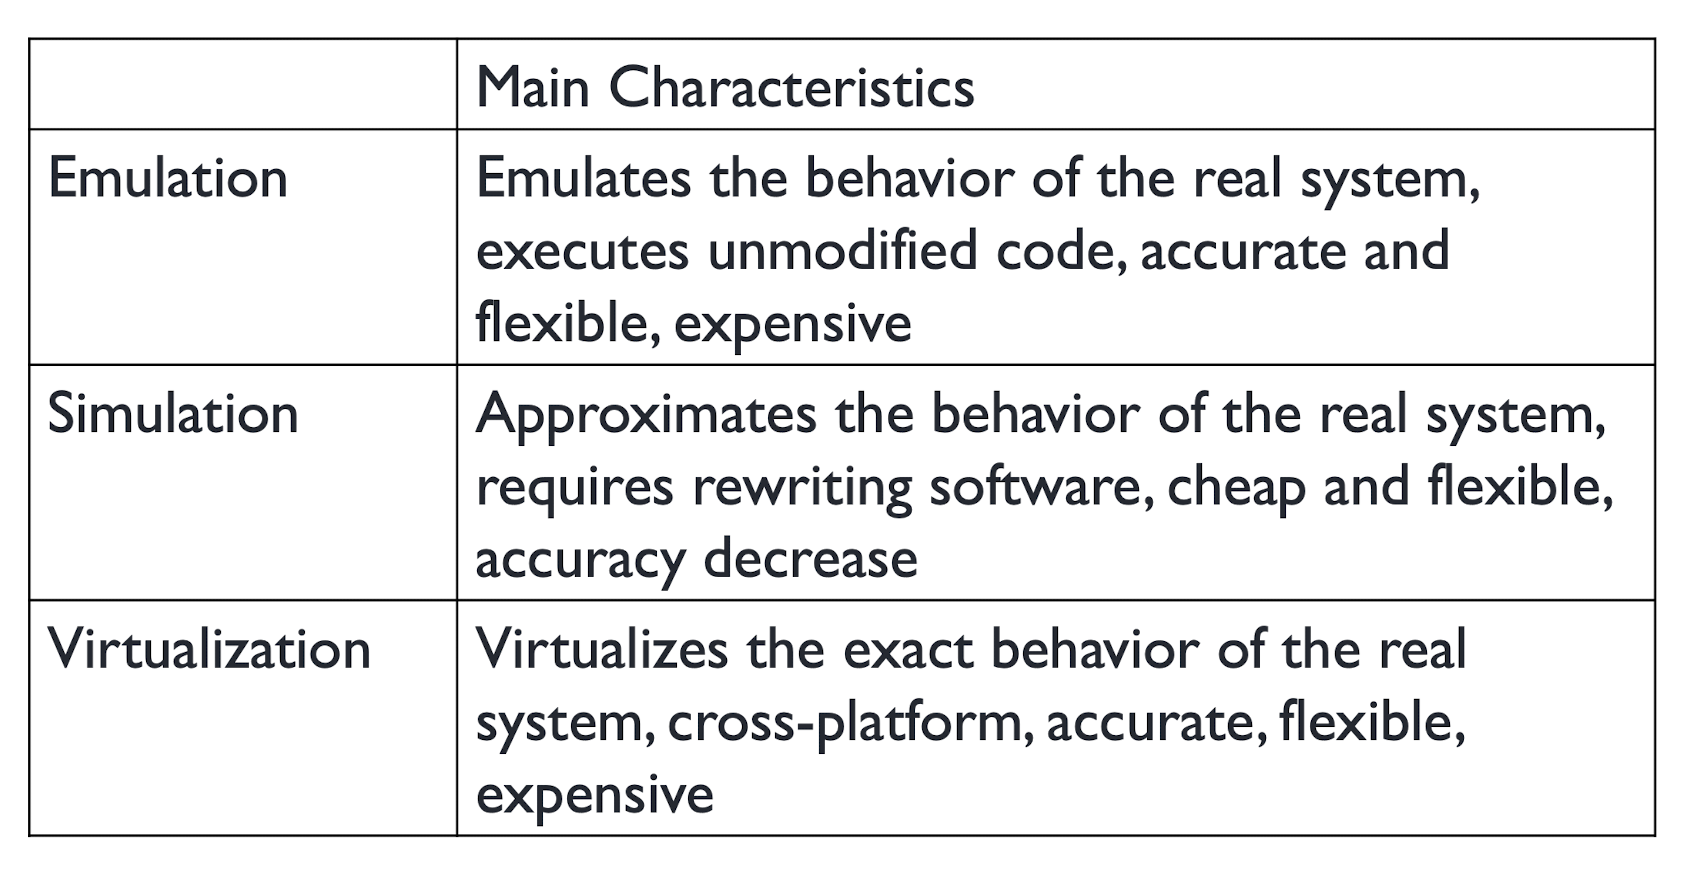
\includegraphics[scale=0.4]{img/summary_virtualization.png}
    \caption{Summary of the principal characteristics of virtualization techniques}
\end{figure}
Now we will focus on each one separately.
\section{Virtualization}
Virtualization is compatible with x86/64 machines, each virtual machine:
\begin{itemize}
    \item Has a full and dedicated environment (encapsulation).
    \item Is isolated from each other just like physical separation (isolation).
    \item Independent from underlying hardware (independence).
    \item Created using existing hardware (partitioning).
\end{itemize}
Virtualization was created to solve some issues:
\begin{itemize}
    \item Too many servers but small workloads
    \item Old hardware does not work
    \item Infrastructural requirements are always increasing (many independent servers)
    \item Small flexibility in shared environments
\end{itemize}
Virtualization allows to keep the costs low for resources while managing them efficiently and keeping the necessary computational power. We can, in fact, use a single hardware server as a multitude of virtual servers.

If a cloud solution has been deployed well we can use virtualization to increase resource usage and enable dynamic sharing of resource pools. We can even react to particular situations because virtualization allows us to have a single consolidated view of each resource of the network which can be easily accessed, moved and managed from wherever.

Other reasons that support the choice of going virtualized are the following:
\begin{itemize}
    \item Better performance
    \item transparency
    \item Heterogeneity
    \item Portability
    \item Interoperability
    \item Green IT (with the same amount of hardware we satisfy more people)
\end{itemize}
Virtualization can be used in many different scenarios, it's heavily used in cloud-based applications because we can, for example, virtualize resources into pools and assign them to users based on the fee they pay and on their workload.

We can also use virtualization to deploy microservice-based applications by putting every microservice into its own virtualized container.

As a last example we can use virtualization to keep our systems secure, with a virtualized environment we can test code and / or applications to see that they work / do not contain viruses before downloading them on our own machine.

A couple of reasons against virtualization are the follwing:
\begin{itemize}
    \item Analysis and planning: building an application or a service that stands on top of a virtualized environment is easy enough, porting something to a virtualized environment a completely different workflow. A lot of planning and study has to go into the process, the staff needs to be trained and a lot of risk analysis has to be done.
    \item Adaptation and post adaptation: A lot of evaluation needs to go into studying the relaiability, the performance, the efficiency and the security of the virtualized environment that will be used.
    \item Maintenance: Maintenance must be kept in mind as well, mostly scalability and security.
\end{itemize}
\begin{figure}
    \centering
    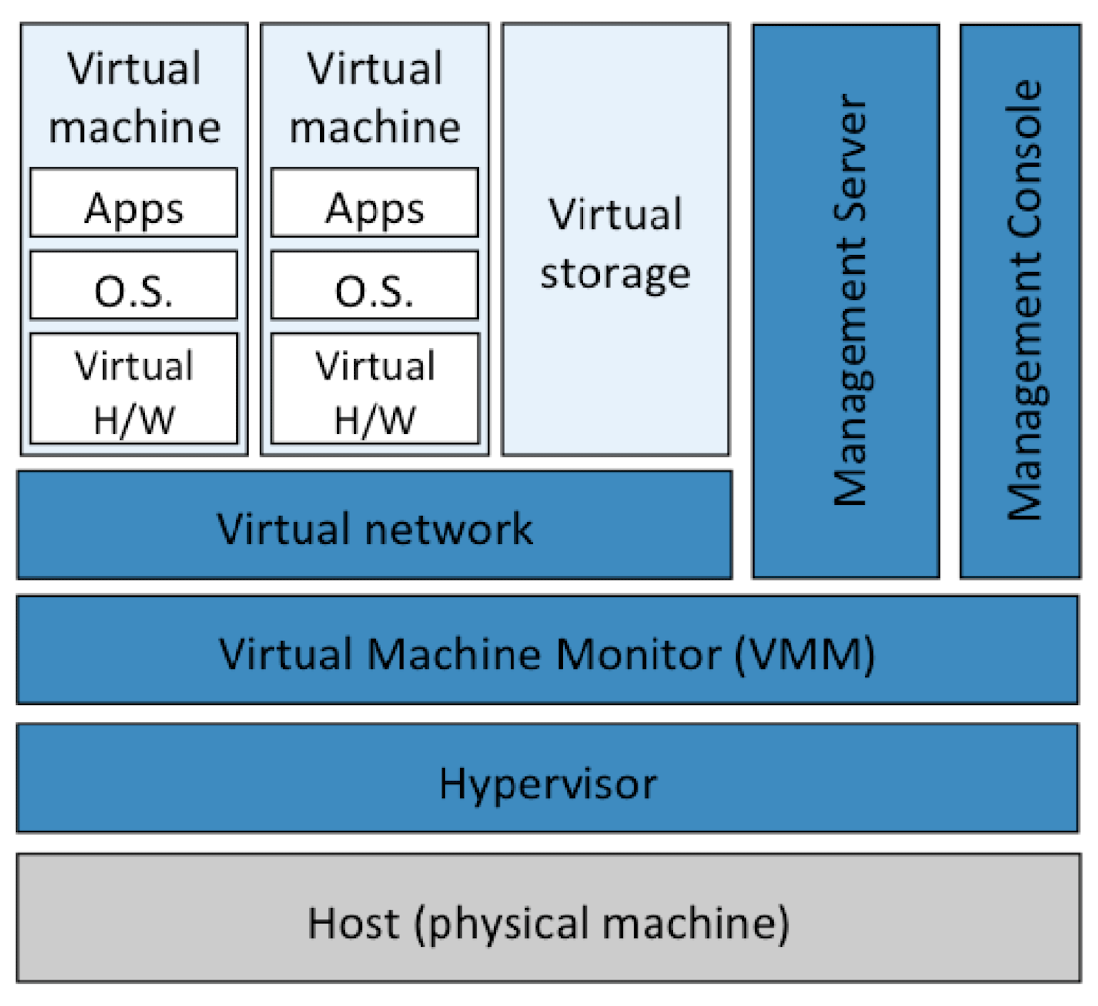
\includegraphics[scale=0.4]{img/virtualization_components.png}
    \caption{The structure of a virtualizer}
\end{figure}
In the following section we will be considering the structure of the virtualizer
\subsection{Virtualizer}
A virtualizer, also known as a hypervisor, is a software layer that enables the creation and management of virtual machines (VMs) on a physical computer. The primary function of a virtualizer is to abstract the underlying hardware resources of a physical machine and allocate them to multiple virtual machines, allowing each VM to operate as if it were running on its own dedicated hardware.

A virtualizer contains the following components:
\begin{itemize}
    \item \textbf{Hypervisor} - The Hypervisor is a component that interacts with the virtual machine and with the host, it allows for multiple OSs running on the same computer. Beware! In the case of an operating system like windows it's important to keep in mind that turning on the Hypervisor and having a virtual machine manager like Virtual Box or VMware may cause instabilities.
    \item \textbf{Virtual machine monitor} - It's the application component realizing virtualization, it must satisfy three properties: Equivalence (the behaviour of the guest OS must be identical to the one of the host OS), Resource control (VMM must have complete control of the resources of the host OS), Efficiency.
    \item \textbf{Guest OS} - The virtualized system.
    \item \textbf{Host OS} - The operating system of the physical machine.
    \item \textbf{Management Server} - It's a virtualization platform, made up of a set of components for managing virtual machines, consolidating servers, allocating resources, migrations and high availability.
    \item \textbf{Management Console} - It's the interface to the virtualization management.
    \item \textbf{Network components} - Enables developing virtual networks comopsed of network devices that are completely controlled through socket and network protocols are simulated in order to replicate the physical ones.
    \item \textbf{Storage components} - It's the storage system of the virtualized environment.
\end{itemize}
A cool factoid about virtualization is that there is a non-mandatory constraint that requires that a statistically relevant percentage of instructions inside a virtualized environment should be executed without virtualization. Abiding to this rule will guarantee better efficiency of the virtual machine.

\subsection{Virtualization Taxonomy}
Popek and Goldberg came up with a series of efficiency requirements that are, to this day, the starting points to determine the sufficient conditions on the hardware architecture that will support the virtualization process. In the definitions (that are lexically a bit dated but still valid, as I said) they refer to the so called "third generation computer", which is none other than the computer that we know today, the system that moved from using transistors to using integrated circuits.
\begin{theorem}
    For any conventional third generation computer, a virtual machine monitor may be constructed (and is efficient) if the set of sensitive instructions for that computer is a subset of privileged instructions (trap in user mode).
\end{theorem}
In other words we are asking that all instructions that can alter the functioning of the system are executed in privileged mode, through an exception, while all non-privileged instructions are natively executed (the theorem is a necessary - sufficient condition).

Since we need to be able to differenciate between different types of instructions we also have an hierarchy:
\begin{itemize}
    \item Privileged instructions - They raise an exception if executed in user mode.
    \item Sensitive instructions (control) - Try to modify the configurations of system resources (global system state).
    \item Sensitive instructions (behavior) - Their result depends on the configuration of system resources (global system state).
\end{itemize}
\begin{theorem}
    A conventional third generation computer is recursively virtualizable if it is virtualizable in an efficient way and a VMM without any timing dependencies can be constructed for it.
\end{theorem}
All virtualization approaches are built on Popek and Goldberg conditions, even though initial implementations of x86 did not meet Popek and Goldberg conditions, these conditions are overall sufficient but not necessary and therefore they could be relaxed to reach different approaches.

Now we will consider different approaches for emulation, simulation and virtualization. These solutions can be found in Figure \ref{fig:virtualization-stacks}.
\begin{figure}
    \centering
    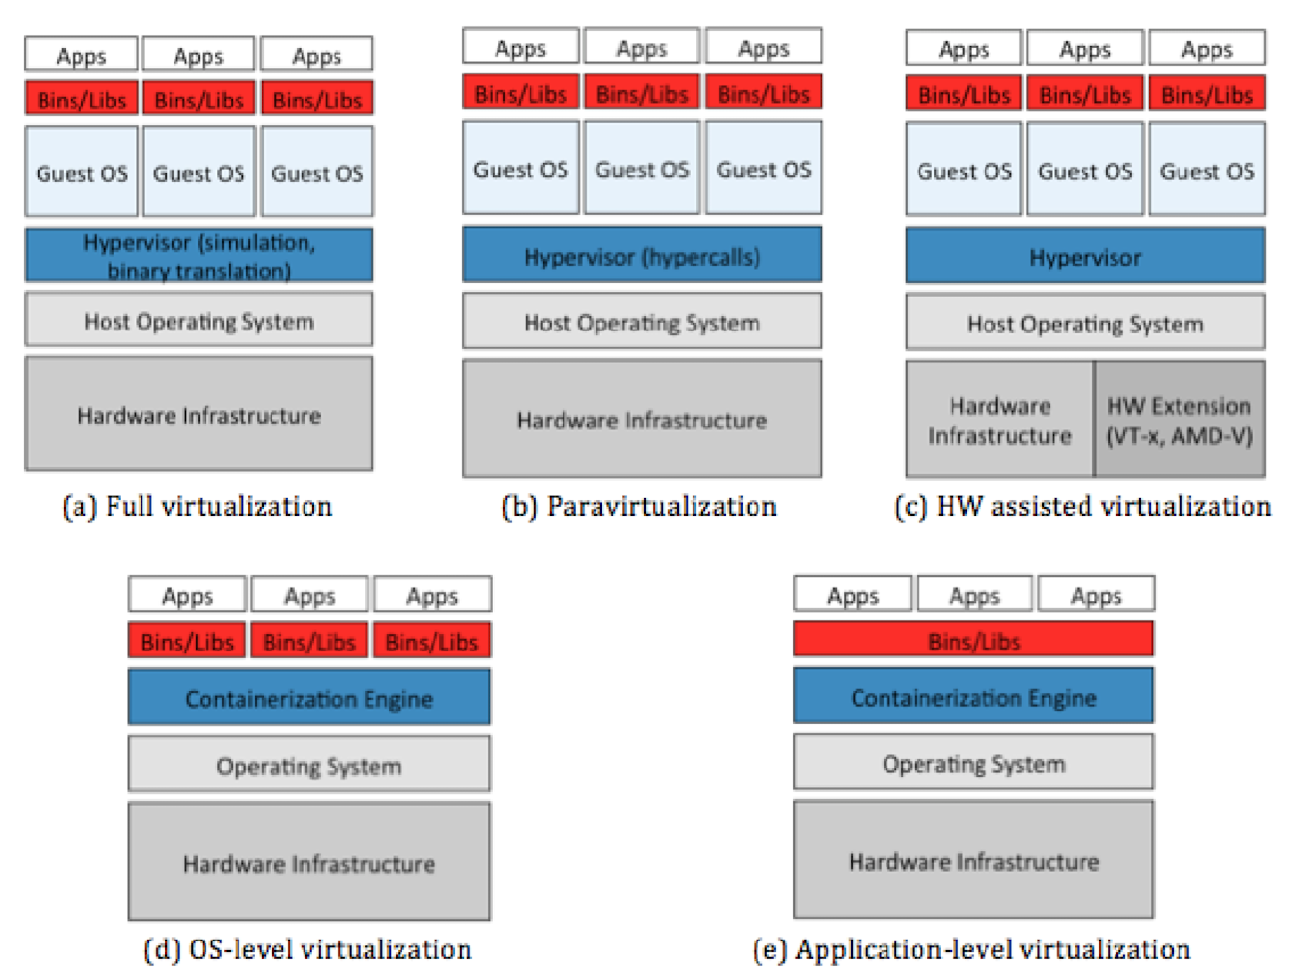
\includegraphics[scale=0.4]{img/virtualization_stacks.png}
    \caption{Various virtualization models}
    \label{fig:virtualization-stacks}
\end{figure}
\begin{itemize}
    \item \textbf{Full emulation} - We emulate every aspect of a computer and it allows to execute an unmodified guest OS on a completely different host architecture.
    \item \textbf{Full virtualization [\ref{fig:virtualization-stacks}.a]} - Only emulates the necessary hardware, allowing the isolated execution of a guest OS, the only difference is that the guest OS must be designed for the same architecture.

    If we need to run software for MIPS-32 architecture we are going to need to emulate the whole machine because we cannot run a virtual machine made for something like that on x86.

    Nowadays processors come with instructions that allow to provide the virtual machine with some true hardware (\textbf{Hardware assisted virtualization} [\ref{fig:virtualization-stacks}.c]). That boosts machine performance with full virtualization, basically a CPU execution targeting privileged instructions allows the VMM to run in a new root mode below the Guest OS level and there is the possibility to do direct execution of user requests to the Host system hardware, therefore there is no need for either binary translation or paravirtualization.
    \item \textbf{Paravirtualization [\ref{fig:virtualization-stacks}.b]} - is another form of virtualization where the virtual machine makes available an API to extend the guest OS (the guest OS has to be modified), the extension consists of hypercall implementation which is a virtualized version of a system call. Basically it's a way of opening a direct line of communication between the Guest OS and the Hypervisor below.
    \item \textbf{OS-level virtualization [\ref{fig:virtualization-stacks}.d]} - the virtual machine manager partitions hardware resources of host OS between the guests. The host OS guarantees the isolation of multiple user space instances, an example of this is Docker.
    \item \textbf{Application level virtualization [\ref{fig:virtualization-stacks}.e]} - we have a virtualized application that runs in a safe and enclosed environment, this avoids risky memory overwrites that may break the operating system. This also allows for better portability of code.
\end{itemize}
Virtualization can either be native or non-native, if it's native is fast because guest OS and host OS coincide and, probably, the Hypervisor is very low level and very efficient. In the other case we are working with a slower form of virtualization but it allows to have different operating systems.

\section{Virtualization Software}
Now we will se a couple of specific solutions for hardware virtualization.
\subsection{VMware ESXi}
The first virtualization platform that we'll check out is vSphere, which is an ecosystem including different virtualization solutions.
\begin{figure}
    \centering
    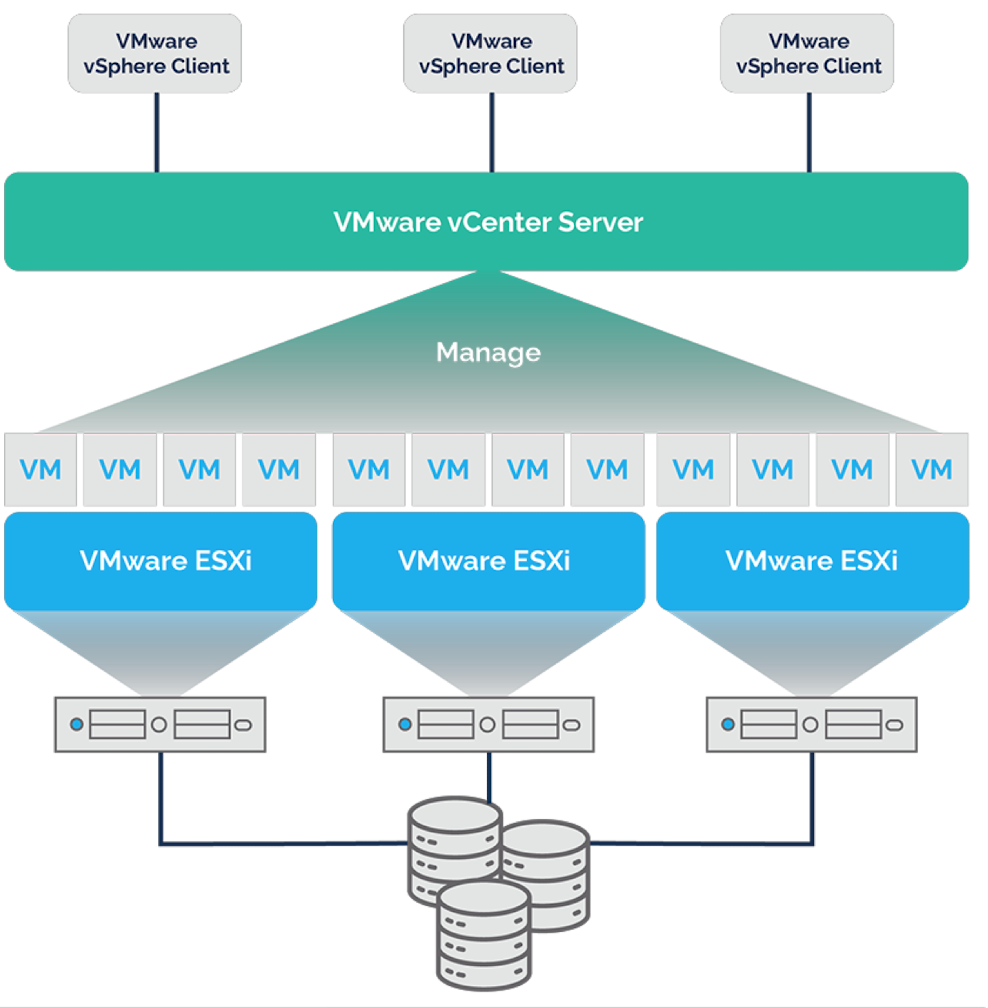
\includegraphics[scale=0.4]{img/ESXi.png}
    \caption{VMware vSphere}
\end{figure}
vCenter is a management middleware layed on top of the virtualized environment and basically allows full control over the resources. This solution allows to control up to 2.000 hosts and 35.000 virtual machines.

ESXi is the vSphere's hypervisor and gives the fundamentals to build and manage a virtualized IT infrastructure. It's a bare-metal hypervisor, installed directly on server hardware and takes up only 150MB. It partitions the physical server into sveral virtual servers, each virtual machine is a complete system on its own.

Virtual machines can be kept safe via powerful encryption systems and role based access control.
\subsection{Xen}
Xen is a Paravirtualization hypervisor released under GPL2 license, with paravirtualization we can expect performance similar to a non-virtualized machine. It can scale up to monstrous numbers: 4.095 host CPUs with 16Tb of RAM; it's important to note that using paravirtualization the hypervisor supports a maximum of 512 VCPUs with 512Gb of RAM per guest, while using Hardware Virtualization, it supports a maximum of 128 VCPUs and 1Tb of RAM per guest.

Why should we use Xen?
\begin{itemize}
    \item It's reliable.
    \item It's flexible.
    \item It has a very good support for a wide range of operating systems and cloud platforms.
    \item It's secure because of the minimal attack surface.
    \item It's modular.
\end{itemize}
Xen's hypervisor is inserted between the hardware and the OS, there is very low overhead and performance are comparable with a native system ones, it re-utilizes Linux device drivers for simplified management, it's robust against driver failures and can protect guests and the hypervisor from driver failures. On top of the hypervisor run a number of virtual machines known as domains, domain 0 is a special guest that contains the drivers for all the devices in the system. Xen's hypervisor:
\begin{itemize}
    \item Optimizes CPU utilization.
    \item Offers performance and scalability for complex systems.
    \item Offers separation between hypervision execution and OS stack management.
    \item Has interchangeable components.
    \item Offers string isolation between components.
\end{itemize}
\subsection{KVM}
KVM is a full virtualization solution for Linux on x86 hardware, it's based on extensions supporting virtualization and can execute unmodified Linux or Windows images.

Now we are going to move to Virtualization in the field of communicating machines.
\section{Virtual Desktop}
Another very cool use of virtualization is virtual desktop, in this case we basically have remote resources and users can hop into a personal virtual machine just by using a thin client and their own credentials. If on one side we should have a completely seemless desktop experience that should present no differences from a user's prospective, on the other end the provider should be able to guarantee load balance, high availability, scalability and performance for all of its users.

The pros are the following:
\begin{itemize}
    \item Centralized management and security.
    \item Business continuity.
    \item Isolation and standard way of managing ProcessDecreases the need to buy new hardware.
    \item Decreases the time of adding a new image.
    \item Centralized adiminstration of all desktop, eventually located anywhere in the world.
\end{itemize}
Virtual desktop can be implemented in a variety of ways dependeing on the type of solution / service desired.
\subsection{Single remote desktop}
Whenever we deal with a single remote desktop we basically remote into our own PC (the remote PC is a blade server located in a datacenter), it's widely used by IT management companies to handle problems on remote machines.

The pros and cons of this kind of model are the following:
\begin{itemize}
    \item Each user has his own PC, instead of sharing resources with other users.
    \item Terminal servers hosting shared desktops can be influenced by server faults/problems.
    \item Blades require more maintenance.
\end{itemize}
\subsection{Virtual desktop machines}
A virtual desktop is the opposite of a shared desktop, a single client -PC or notebook- hosts multiple desktops, each one with its own operating system.
\subsection{Shared Desktops}
Shared desktops are based upon a server hosting desktop users and applictaions, desktop sharing is widely used because all the computing power is located on a server and only the monitor, keyboard and mouse are connected to the network.

This system allows a centralized management of desktops and their applications, simplifying licensing and making easier to solve problems, because user applications are located on the server and not on several machines.
\subsection{VDI central hosting}
Any user can connect through a thing client and a gateway to a broker that is able to fetch the requested image from an image server which is then sent to another set of servers that are used to run the image, obviously it's working in a virtualized environment and therefore the hosts are actually virtual machines running on one or more servers.
\section{Server Virtualization}
Server virtualization decreases the total cost of ownership because it allows to serve more clients with the same amount of computational power. It also allows to increase server usage and simplifies management via:
\begin{itemize}
    \item Dynamic provisioning
    \item Workload managment and isolation
    \item Virtual machine migration
    \item Reconfiguration
\end{itemize}
\textbf{Blade physical desktops}
Users have their own PC, but the physical hardware is a blade PC located in a datacenter. The main pros and cons of this approach are the following:
\begin{itemize}
    \item Each user has his own PC, instead of sharing resources with other users.
    \item Terminal servers hosting shared desktops can be influenced by server faults/problems.
    \item Blades require more maintenance.
\end{itemize}
